\documentclass{article}
    \usepackage{amssymb}
    \usepackage[utf8]{inputenc}
    \usepackage[russian]{babel}
    \usepackage[left=2cm,right=2cm,
        top=2cm,bottom=2cm,bindingoffset=0cm]{geometry}
    \usepackage{hyperref}
    \hypersetup{
        colorlinks=true,
        linkcolor=blue,
        filecolor=magenta,      
        urlcolor=cyan,
    }
  \usepackage{graphicx}
  \graphicspath{{pictures/}}
  \DeclareGraphicsExtensions{.pdf,.png,.jpg}

\begin{document}
\begin{center}{\hugeОтчет по курсовой работе за неделю\\}\end{center}
Дата: 25.9.2020\\
Научные руководители: Герасимов С.В., Мещеряков А.В.\\
Студент: Немешаева Алиса\\
Курс: 4\\

\renewcommand{\labelitemi}{$\blacksquare$}
\renewcommand\labelitemii{$\square$}
\begin{enumerate}
    \item На этой неделе продолжалось обучение модели для повторения результатов выбранной статьи. 
        Был добавлен еще один каталог скоплений для проверки верности детекции.\\
    
    \begin{table}[h!]
        \begin{tabular}{p{0.45\linewidth}p{0.45\linewidth}}
            \textbf{40 эпох} & \textbf{14 эпох}\\
            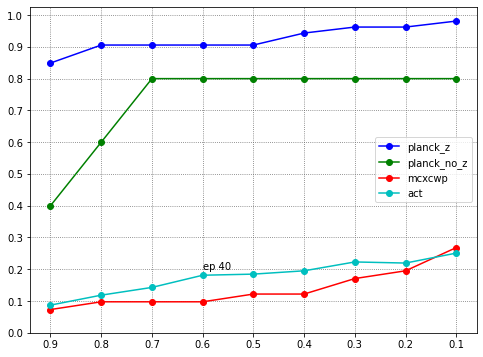
\includegraphics[width=\linewidth]{recall40} & 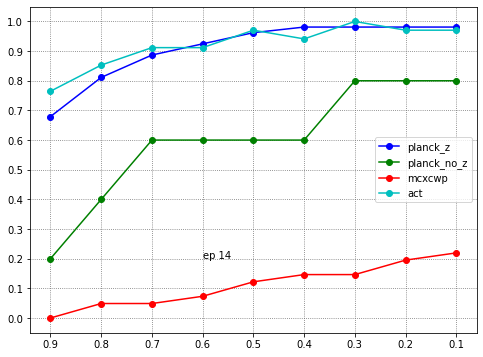
\includegraphics[width=\linewidth]{recall14}\\ 
            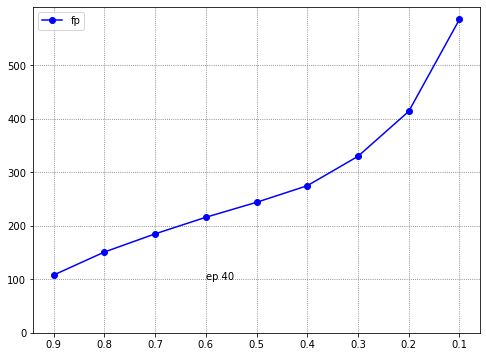
\includegraphics[width=\linewidth]{fp40} & 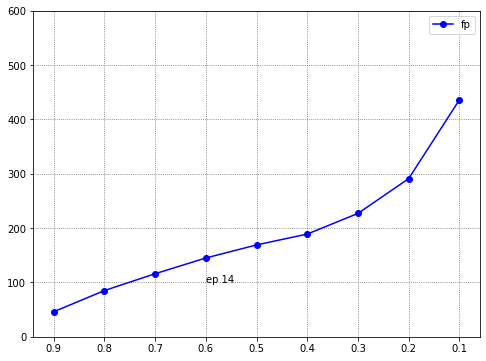
\includegraphics[width=\linewidth]{fp14}\\ 
        \end{tabular}
    \end{table}

    \item Кроме того, в алгоритм детекции был добавлен новый метод определения центров скоплений на 
        выходе нейросети. Старый метод искал центры на маске из единиц, новый метод учитывает 
        prediction index (значение маски на выходе из нейросети). Проведено сравнение методов на 
        разных моделях.\\

    \begin{table}[h!]
        \begin{tabular}{p{0.45\linewidth}p{0.45\linewidth}}
            \textbf{Бинарные маски} & \textbf{Маски с сохранёнными prediction index}\\
            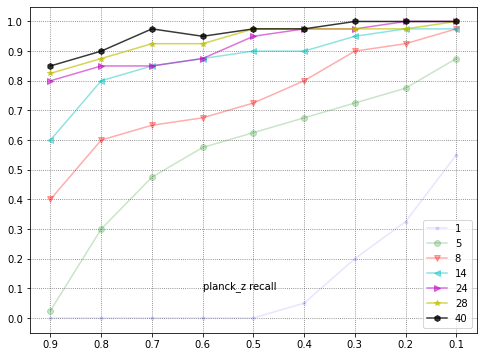
\includegraphics[width=\linewidth]{p} & 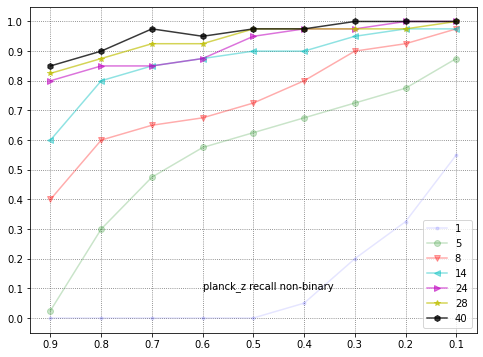
\includegraphics[width=\linewidth]{p_non_binary}\\ 
            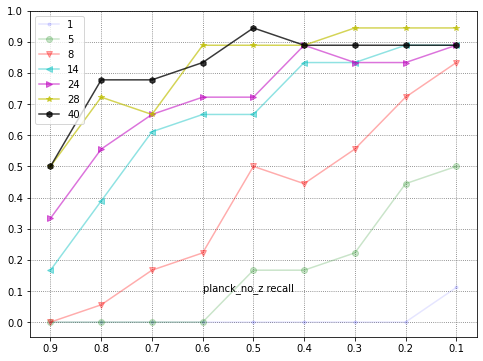
\includegraphics[width=\linewidth]{pnz} & 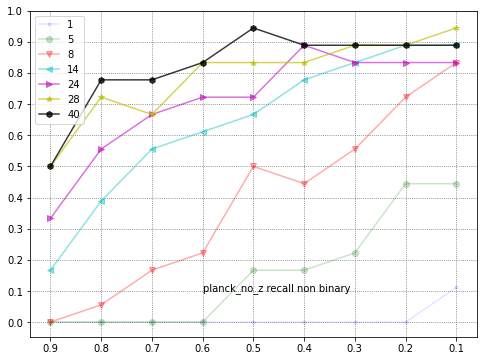
\includegraphics[width=\linewidth]{pnz_non_binary}\\ 
            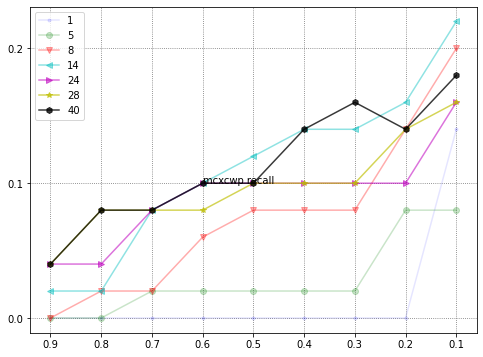
\includegraphics[width=\linewidth]{m} & 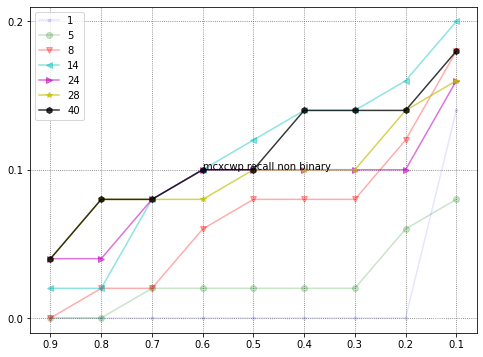
\includegraphics[width=\linewidth]{m_non_binary}\\ 
            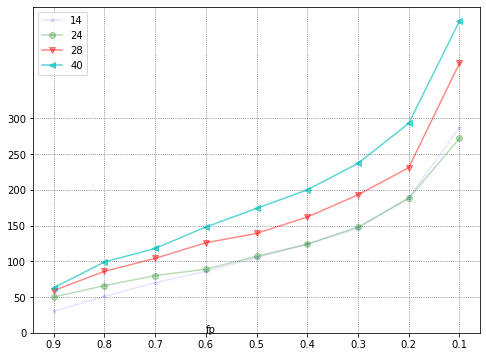
\includegraphics[width=\linewidth]{fp1} & 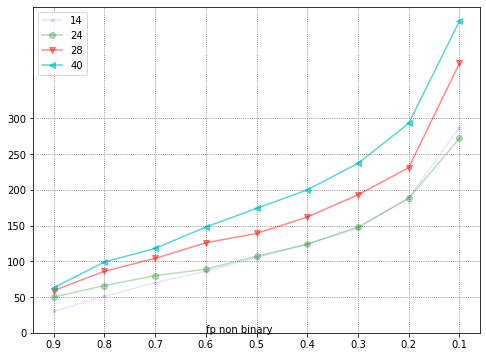
\includegraphics[width=\linewidth]{fp1_non_binary}\\ 
        \end{tabular}
    \end{table}
\end{enumerate}

Общее количество строк кода за эту неделю: 199\\
\end{document}
